% The orthogonality condition of the talk, in the notation of the 2026-09-25 meeting
% (Phi = d f_base / d theta on the data, Delta = the learned correction), each symbol
% labelled in words. The full formulas are in orthogonality_formulas.tex (backup slide).
\documentclass[border=8pt]{standalone}
% Shared preamble of the TikZ slide figures. Role colours match style.py.
\usepackage[T1]{fontenc}
\usepackage[scaled]{helvet}
\renewcommand\familydefault{\sfdefault}
\usepackage{amsmath}
\usepackage{tikz}
\usetikzlibrary{arrows.meta,calc,decorations.pathmorphing,positioning}
\definecolor{cbase}{HTML}{D55E00}   % physics model
\definecolor{caug}{HTML}{0072B2}    % augmented model, no projection
\definecolor{cproj}{HTML}{009E73}   % augmented model with projection
\definecolor{cink}{HTML}{222222}
\definecolor{cmuted}{HTML}{6B6B6B}

\begin{document}
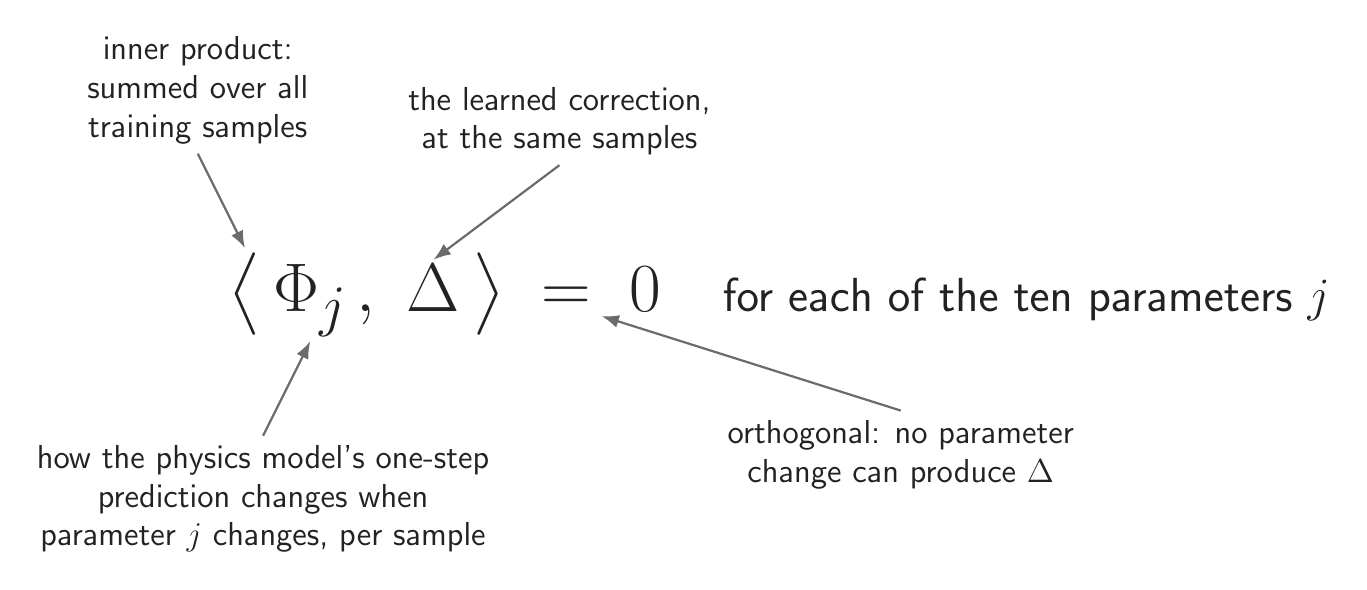
\begin{tikzpicture}[
    t/.style={inner sep=1.5pt, font=\Huge, text=cink},
    lab/.style={font=\large, align=center, text=cink},
    pt/.style={-{Latex[length=2.2mm]}, cmuted, line width=0.8pt}]
  \node[t] (la) {$\big\langle$};
  \node[t, base right=1pt of la] (P) {$\Phi_j$};
  \node[t, base right=0pt of P] (c) {$,$};
  \node[t, base right=8pt of c] (D) {$\Delta$};
  \node[t, base right=1pt of D] (ra) {$\big\rangle$};
  \node[t, base right=10pt of ra] (eq) {$=\;0$};
  \node[font=\LARGE, text=cink, anchor=base west] at ($(eq.base east)+(6mm,0)$)
       {for each of the ten parameters $j$};

  \node[lab, above=12mm of la, xshift=-6mm] (lI) {inner product:\\summed over all\\training samples};
  \node[lab, below=12mm of P, xshift=-6mm] (lP) {how the physics model's one-step\\prediction changes when\\parameter $j$ changes, per sample};
  \node[lab, above=12mm of D, xshift=16mm] (lD) {the learned correction,\\at the same samples};
  \node[lab, below=12mm of eq, xshift=38mm] (lE) {orthogonal: no parameter\\change can produce $\Delta$};
  \draw[pt] (lI.south) -- (la.north);
  \draw[pt] (lP.north) -- (P.south);
  \draw[pt] (lD.south) -- (D.north);
  \draw[pt] (lE.north) -- (eq.south);
\end{tikzpicture}
\end{document}
